\documentclass{article}

\usepackage{geometry}
\usepackage{amsmath}
\usepackage{mathtools}
\usepackage{amsfonts}
\usepackage{hyperref}
\usepackage{color}
\usepackage{tikz}
\usetikzlibrary{graphs, arrows.meta, positioning}
\usepackage{algorithm}
\usepackage[noend]{algpseudocode}
\usepackage{graphicx}

\hypersetup{
    colorlinks=true, %set true if you want colored links
    linktoc=all,     %set to all if you want both sections and subsections linked
    linkcolor=black,  %choose some color if you want links to stand out
}
\geometry{
    a4paper, % Paper size
    left=2cm, % Left margin
    right=2cm, % Right margin
    top=2cm, % Top margin
    bottom=2cm, % Bottom margin
}

\title{Teoremi Informatica Teorica}
\author{Zbirciog Ionut Georgian}
\date{\today}

\renewcommand{\contentsname}{Indice}

\begin{document}
\maketitle

\begin{flushleft}

\tableofcontents
\newpage

\section{Teoremi Dispensa 2}

\subsection{Teorema a pag. 5}
Per ogni macchina di Turing non deterministica $NT$ esiste una macchina di Turing detreministica $T$
tale che, per ogni possibile input $x$ di $NT$ , l'esito della computazione $NT(x)$ coincide con l'esito della computazione
di $T(x)$.

\paragraph*{Dimostrazione:}
Eseguiamo una simulazione della macchina non deterministica $NT$ mediante una macchina deterministica $T$. La simulazione consiste 
in una visita in ampiezza\footnote{Perché non in profondità? Non possiamo fare una visità in profondità perché non sappiamo la lunghezza di ciascuna computazione, in quanto potrebbero
anche non finire.} dell'albero delle computazioni di $NT$ basata sulla tecnica \textit{coda di rondine con ripetizioni}.
Partiamo dallo stato globale $SG(T, x, 0)$ e simuliamo tutte le computazione di lunghezza 1. Se tutte le computazioni terminano in 
$q_{R}$ allora $T$ rigetta, se almeno una computazione termina in $q_{A}$ allora $T$ accetta, altrimenti ricominciamo da capo 
eseguendo tutte le computazioni di lunghezza 2 e così via.
\section{Teoremi Dispensa 3}

\subsection{Teorema a pag. 3}

Un linguaggio $L \subseteq \Sigma^{\star}$ è decidibile se e soltanto se $L$ e $L^{c}$ sono accettabili.

\paragraph*{Dimostrazione:}
\begin{itemize}
    \item[$(\Rightarrow$]{
        Se $L$ è decidibile allora esiste una macchina di Turing $T$ deterministica tale che $\forall x\in\ \Sigma^{\star}$, $T(x) = q_{A} \Leftrightarrow\ x\in L \land T(x) = q_{R} \Leftrightarrow\ x\in L^{c}$.
        Osserviamo dunque che $T$ accetta $L$.
        
        Da $T$, deriviamo ora $T^{'}$ aggiungendo le seguenti quintuple: 
        $$
        \langle q_{A}, x, x, q_{R}^{'}, stop \rangle \land \langle q_{R}, x, x, q_{A}^{'}, stop \rangle\ \forall x \in \Sigma \cup \square
        $$
        L'esecuzione di $T^{'}$ è simile a quella di $T$, solo che gli stati di accettazione e rigetto sono stati invertiti, in questo modo
        se $T$ accetta $x$ allora $T^{'}$ rigetta $x$, mentre se $T$ rigetta $x$, $T^{'}$ accetta $x$, dunque $T{'}$ accetta $L^{c}$.
    }
    \item[$\Leftarrow)$]{
        Se $L$ e $L^{c}$ sono accettabili allora esistono due macchine di Turing $T_{1}$ e $T_{2}$ tali che, $\forall x\in \Sigma^{\star}\, T_{1}(x) = q_{A} \Leftrightarrow x\in L \land T_{2}(x) = q_{A} \Leftrightarrow x\in L^{c}$.
        Non esendo specificato l'esito della computazione nel caso in cui $x \notin L$ e $x \notin L^{c}$ definiamo la macchina 
        $T$ che, simulando $T_{1}$ e $T_{2}$ decide $L$ nel seguento modo\footnote{Osserviamo che non possiamo simulare $T_{1}$ e $T_{2}$ "blackbox", in quanto non sappiamo se la loro computazione termina o meno.}:
        \begin{enumerate}
            \item Esegui una singola istruzione di $T_{1}$ sul nastro 1: se $T_{1}(x) = q_{A}$ allora $T(x) = q_{A}$, altrimenti esegui il passo (2).
            \item Esegui una singola istruzione di $T_{2}$ sul nastro 2: se $T_{2}(x) = q_{A}$ allora $T(x) = q_{R}$, altrimenti esegui il passo (1).
        \end{enumerate}   
        Se $x \in L$, allora prima o poi, al passo $(1),\ T_{1}$ entrerà nello stato di accettazione, portando $T$ ad accettare.\\
        Se $x \in L^{c}$, allora prima o poi, al passo $(1),\ T_{1}$ entrerà nello stato di accettazione, portando $T$ a rigettare.
    }
\end{itemize}

\subsection{Teorema a pag. 4}
Un linguaggio $L$ è decidibile se e soltanto se la funzione $\chi_{L}$ è calcolabile.

\paragraph*{Dimostrazione:}
\begin{itemize}
    \item[$(\Rightarrow$]{
        Se $L$ è decidibile allora esiste una macchina di Turing $T$ deterministica di tipo \textbf{riconoscitore} tale che $\forall x\in\ \Sigma^{\star}$, $T(x) = q_{A} \Leftrightarrow\ x\in L \land T(x) = q_{R} \Leftrightarrow\ x\in L^{c}$.
        A partire da $T$ definiamo una macchina di Turing $T^{'}$ di tipo trasduttore a 2 natri, con input $x\in\Sigma^{\star}$ che opera nel seguente modo:
        \begin{enumerate}
            \item Sul primo nastro simula $T(x)$.
            \item Se $T(x)$ termina nello stato $q_{A}$ allora $T{'}(x)$ scrive sul nastro di output il valore 1, altrimenti scrive il valore 0 e poi termina.
        \end{enumerate}
        Osserviamo che poiché $L$ è decidibile il passo (1) termina sempre per ogni input $x$. Se $x\in L$ allora $T(x) = q_{A}$ e $T^{'}(x)$ scrive 1 sul nastro di output.
        Se $x\notin L$ allora $T(x) = q_{R}$ e $T^{'}(x)$ scrive 0 sul nastro di output. Questo dimostra che $\chi_{L}$ è calcolabile.
    }
    \item[$\Leftarrow)$]{
        Se $\chi_{L}$ è calcolabile e per costruzione anche totale allora esiste una macchina di Turing $T$ di tipo \textbf{trasduttore}, che per ogni $x\in \Sigma^{\star}$, calcola $\chi_{L}(x)$.
        A partire da $T$ definiamo $T^{'}$ di tipo riconoscitore a 2 natri, con input $x\in\Sigma^{\star}$ che opera nel seguente modo:
        \begin{enumerate}
            \item Sul primo nastro simula $T(x)$ scrivendo il risultato sul secondo nastro.
            \item Se sul secondo nastro c'é scritto 1 allora $T^{'}(x) = q_{A}$, altrimenti nello stato $q_{R}$.
        \end{enumerate}
        Osserviamo che poiché $\chi_{L}$ è calcolabile il passo (1) termina sempre per ogni input $x$. Se $\chi_{L}(x) = 1$ allora (1) termina scrivendo 1 sul secondo nastro e $T^{'}(x) = q_{A}$.
        Se $\chi_{L}(x) = 0$ allora (1) termina scrivendo 0 sul secondo nastro e $T^{'}(x) = q_{R}$. Questo dimostra che $L$ è decidibile.
    }
\end{itemize}
\newpage
\subsection{Teorema a pag. 5}

Se la funzione $f: \Sigma^{\star}\rightarrow\Sigma^{\star}_{1}$ è totale e calcolabile allora il linguaggio $L_{f}\subseteq\Sigma^{\star} \times \Sigma^{\star}_{1}$ è decidibile.

\paragraph*{Dimostrazione:}
Poiché $f$ è calcolabile e totale allora esiste una macchina di Turing trasduttore che calcola $f(x) \forall x\in \Sigma^{\star}$. A partire da $T$
definiamo una macchina di Turing $T^{'}$ riconoscitore a due nastri con input $\langle x, y \rangle$ dove $x\in \Sigma^{\star}$ e $y\in \Sigma^{\star}_{1}$, che opera nel seguente modo:
\begin{enumerate}
    \item Sul nastro 1 è scritto l'input $\langle x, y \rangle$.
    \item Sul nastro 2 simula $T(x)$, scrivendovi il risultato $z$.
    \item Se $z = y$ allora $T^{'}(x) = q_{A}$ altrimenti va in $q_{R}$. 
\end{enumerate}
Osserviamo che, poiché $f$ è totale e calcolabile il passo (2) termina per ogni input $x\in \Sigma{\star}$. Se $f(x) = z = y$ allora $T^{'}(x)$ termina in $q_{A}$.
Se $f(x) = z \neq y$ allora $T^{'}(x)$ termina in $q_{R}$. Questo dimostra che $L_{f}$ è decidibile.

\subsection{Teorema a pag. 5}

Sia $f: \Sigma^{\star}\rightarrow\Sigma^{\star}_{1}$ una funzione. Se il linguaggio $L_{f}\subseteq\Sigma^{\star} \times \Sigma^{\star}_{1}$ è decidibile allora $f$ è calcolabile\footnote{Osserviamo che non possiamo invertire del tutto il teorema precendente, dalla decidibilità di $L_{f}$ possiamo dedurre solo la calcolabilità di $f$}.

\paragraph*{Dimostrazione:}

Poiché $L_{f}\subseteq\Sigma^{\star} \times \Sigma^{\star}_{1}$ è decidibile, esiste una macchina di Turing riconoscitore $T$, tale che $\forall x\in \Sigma^{\star}$ e $\forall y\in \Sigma^{\star}_{1}$,
$T(x) = q_{A}$ se $y = f(x)$ e $T(x) = q_{R}$ se $y \neq f(x)$. A partire da $T$ definiamo una macchina di Turing trasduttore $T^{'}$ con input $x\in \Sigma^{\star}$ che opera nel seguente modo:
\begin{enumerate}
    \item Scrive $i = 0$ sul nastro 1.
    \item {
        Enumera tutte le stringhe $y\in \Sigma^{\star}_{1}$ di lunghezza pari al valore scritto sul primo nastro, simulando per ciascuna stringa $T(x, y)$.
        \begin{enumerate}
            \item Sia $y$ la prima stringa di lunghezza $i$ non ancora enumerata, allora scrive $y$ sul secondo nastro.
            \item Sul terzo nastro, esegue la computazione $T(x, y)$.
            \item Se $T(x, y) = q_{A}$ allora scrive $y$ sul nastro di output eventualmente incrementando $i$ se $y$ era l'ultima stringa, torna al passo (2). 
        \end{enumerate}
        }
\end{enumerate}

Poiché $L_{f}$ è decidibile il passo (b) termina per ogni input $(x, y)$. Se $x$ appartiene al dominio di $f$, allora $\exists y\in \Sigma^{\star}_{1}$ tale che $y = f(x)$, e quindi $(x, y)\in L_{f}$. Allora prima o poi la strigna $y$ verrà scritta sul secondo nastro
e $T(x, y) = q_{A}$. Questo dimostra che $f$ è calcolabile.

\subsection{Teorema a pag. 7}

Per ogni programma scritto in accordo con il linguaggio di programmazione \textbf{PascalMinimo}, esiste un macchina di Turing $T$ di tipo trasduttore che scrive sul nastro di output lo stesso valore fornito in output dal programma.

\paragraph*{Dimostrazione omessa}

\subsection{Teorema a pag. 9}

Per ogni macchina di Turing deterministica $T$ di tipo riconoscitore ad un nastro esiste un programma $P$ scritto in accordo alle regole
del linguaggio \textbf{PascalMinimo} tale che, per ogni stringa $x$, se $T(x)$ termina nello stato fiale $q_{F}\in\{q_{A}, q_{R}\}$ allora $P$ con input 
$x$ restituisce $q_{F}$ in output.

\paragraph*{Dimostrazione omessa}
\section{Teoremi Dispensa 5}

\subsection{Teorema a pag. 2}

L'insieme $T$ delle macchine di Turing definite sull'alfabeto $\{0, 1\}$ e dotate di un singolo nastro
(più l'eventuale nastro di output) è numerabile

\paragraph*{Dimostrazione:}
Per dimostrare tale teorema, dobbiamo trovare una biezione tra l'insieme $T$ e l'insieme $\mathbb{N}$. Tale 
biezione non è altro che una etichettatura degli elementi dell'insieme con etichette appartenenti ad $\mathbb{N}$, ossia,
una numerazione degli elementi dell'insieme. Sia $T$ una macchina di Turing e $\beta_{T}$ la sua codifica.

Dunque, rappresentiamo $T$ con la parola $\beta_{T}\in \Sigma^{\star}$, con $\Sigma=\{0, 1, \oplus, \otimes, -, f, s, d\}$ come segue:

$$
\beta_{T} = b(q_{0})\ -\ b(q_{1})\otimes b(q_{11})\ -\ b_{11}\ -\ b_{12}\ -\ b(q_{12})\ -\ m_{1}\oplus \dots \oplus b(q_{h1})\ -\ b_{h1}\ -\ b_{h2}\ -\ b(q_{h2})\ -\ m_{h}
$$

Ora, effettuando le seguenti sostituzione in $\beta_{T}$, otteniamo una stringa in $\mathbb{N}$ 

\begin{itemize}
    \item "s" con "5"
    \item "f" con "6"
    \item "d" con "7"
    \item "-" con "4"
    \item "$\otimes$" con "3"
    \item "$\oplus$" con "2"
\end{itemize}

Inoltre, dato che la stringa può iniziare con un "0", allora premettiamo il carattere "8" alla stringa ottenuta.

La parola in $\{0, 1, 2, 3, 4, 5, 6, 7, 8\}^{\star}$ così ottenuta, può, ovviamente, essere considerata come un numero 
espresso in notazione decimale, ovvero il numero $v(T)\in \mathbb{N}$ associato univocamente a $T$.

\subsection{Teorema a pag. 4 (Halting Problem)}

Definiamo il seguente linguaggio $L_{H}$ in questo modo:
$$L_{H} = \{(i, x): i\ \grave{e}\ la\ codifica\ di\ una\ TM\ \land\ T_{i}(x)\ termina\}$$
Il linguaggio $L_{H}$ è accettabile.

\paragraph*{Dimostrazione:} Dobbiamo dimostrare che esiste una macchina di Turing $T$ tale che, per ogni
input $(i, x ) \in \mathbb{N} \times \mathbb{N}$, $T(i, x) = q_{A}$ se e soltanto se $(i, x) \in L_{H}$.\\ 
Definiamo $U^{'}$ una macchina di Turing universale modificata con input $(i, x)$.
Tale macchina opera nel seguente modo:
\begin{enumerate}
    \item Verifica se $i$ è la codifica di una macchina di Turing. Se non lo è allora $U^{'}(i, x) = q_{R}$.
    \item Simula $U(i, x)$, se termina in $q_{A}$ o in $q_{R}$ allora $U^{'}(x) = q_{A}$.
\end{enumerate}

$U^{'}$ non sa decidere $L_{H}^{c}$, perciò lo accetta solo.

\subsection{Teorema a pag. 4 (Halting Problem)}

Il linguaggio $L_{H}$ non è decidibile

\paragraph*{Dimostrazione:} Supponiamo che $L_{H}$ sia decidibile. Allora, deve esistere una macchina di Turing $T$ tale che, 
$T(i, x) = q_{A} \Leftrightarrow (i, x)\in L_{H}$ e $T(i, x) = q_{R} \Leftrightarrow (i, x)\notin L_{H}$.

\begin{enumerate}
    \item [+]{
        Da $T$ \textbf{deriviamo} $T^{'}$ che terminando su ogni input, accetta tutte e sole le coppie $(i, x) \in \mathbb{N} \times \mathbb{N} \setminus L_{H}$, ossia $L_{H}^{c}$.
        $T^{'}(i, x) = q_{R} \Leftrightarrow (i, x)\in L_{H}$ e $T(i, x) = q_{A} \Leftrightarrow (i, x)\notin L_{H}$.
        Quindi $T^{'}(i, x)$ decide $L_{H}^{c}$.
    }
    \item [+]{
        Da $T^{'}$ \textbf{deriviamo} $T^{''}$ in questo modo:\\
        $T^{''}(i, x) =\ non\ termina\ se\ T^{'}(i, x) = q_{R}$ e $T^{''}(i, x) = q_{A} se\ T^{'}(i, x) = q_{A}$.\\
        Quindi $T^{''}(i, x) =\ non\ termina\ se\ (i, x) = \in L_{H}$ e $T^{''}(i, x) = q_{A}\ se\ (i, x) \notin L_{H}$.
    }
    \item [+]{
        Da $T^{''}$ \textbf{deriviamo} $T^{*}$ in questo modo:\\
        $T^{*}(i) = T^{''} = \ non\ termina\ se\ (i, i) \in L_{H}$ e $T^{*}(i) = T^{''}(i, i) = q_{A}\ se\ (i, i) \notin L_{H}$.\\
    }
\end{enumerate}

Se $T$ esiste $\Rightarrow$ $T^{*}$ esiste, allora $\exists k\in \mathbb{N}$ tale che $T^{*} = T_{k}$. Se $T_{k}(k) = T^{*}(k)$ accettasse, allora $T^{'}(k, k)$ dovrebbe accettare
ach'essa. Ma se $T^{'}(k, k)$ accetta, allora $(k, k)\notin L_{H}$, ossia, $T_{k}(k)$ non termina. Allora $T^{*}(k)$ non può accettare e, dunque, necessariamente non termina.
Ma, se $T^{*}(k)$ non termina, allora $T^{'}(k, k)$ rigetta e, quindi, $(k, k)\in L_{H}$. Dunque, per definizione, $T_{k}(k)$ termina. Quindi, in entrambi le ipotesi, $T_{k}(k)$ termina
o non termina, portando ad una contraddizione. Allora $T^{*}$ non può esistere, ma allora neanche $T^{''}$ può esistere, e neanche $T^{'}$ e di conseguenza $T$.
Quindi se $T$ non esiste, $L_{H}$ non è decidibile.

\subsection{Teorema a pag. 6}

Se $L_{1} e L_{2}$ sono due linguaggi accettabili, allora $L_{1} \cup L_{2}$ è un linguaggio accettabile.\\
Se $L_{1} e L_{2}$ sono due linguaggi decidibili, allora $L_{1} \cup L_{2}$ è un linguaggio decidibile.

\paragraph*{Dimostrazione:}

\subsection{Teorema a pag. 6}

Se $L_{1} e L_{2}$ sono due linguaggi accettabili, allora $L_{1} \cap L_{2}$ è un linguaggio accettabile.\\
Se $L_{1} e L_{2}$ sono due linguaggi decidibili, allora $L_{1} \cap L_{2}$ è un linguaggio decidibile.

\paragraph*{Dimostrazione:}

\section{Teoremi Dispensa 6}

\subsection{Teorema a pag. 3}

Sia $T$ una macchina di Turing deterministica, definita su un alfabeto $\Sigma \setminus \square$ e 
un insieme di stati $Q$, e sia $x\in \Sigma^{\star}$ tale che $T(x)$ termina, allora: 
$$dspace(T, x) \leq dtime(T, x) \leq dspace(T, x)|Q|(|\Sigma| + 1)^{dspace(T, x)}$$

\paragraph*{Dimostrazione:} 
\begin{enumerate}
    \item {
        $dspace(T, x) \leq dtime(T, x)$\\
        Banalmente, una computazione deterministica che termina in $k$ passi non può utilizzare più di $k$ celle del nastro.
    }
    \item {
        $dtime(T, x) \leq dspace(T, x)|Q|(|\Sigma| + 1)^{dspace(T, x)}$
        \begin{enumerate}
            \item {
                $dspace(T, x)|Q|(|\Sigma| + 1)^{dspace(T, x)}$: è il numero di stati globali possibili di $T$ nel caso in cui non più di $dspace(T, x)$ celle del nastro 
                vengano utilizzate dalla computazione $T(x)$.
            }
            \item {
                $(|\Sigma| + 1)^{dspace(T, x)}$: sono tutte le possibili parole di $dspace(T, x)$ simboli di $\Sigma \cup \{\square\}$, ossia tutte le possibili
                configurazioni delle $dspace(T, x)$ celle utilizzate.
            }
        \end{enumerate}
        Siano, dunque, $T$ una macchina deterministica e $x\in \Sigma^{\star}$ tali che $T(x)$ termina in $k$ passi utilizzando
        $dspace(T, x)$ celle del nastro. Poiché $T(x)$ termina in $k$ passi, essa è una successione di stati globali 
        $$SG_{0}(x), SG_{2}(x), \dots, SG_{k}(x)$$
        tali che $SG_{0}(x)$ è lo stato globale iniziale e per ogni $0 \leq i \leq k - 1$ esiste una transizione
        $SG_{i}(x) \rightarrow SG_{i + 1}(x)$, e  $SG_{k}(x)$ è lo stato globale finale.\\
        Sia $k(T, x) = dspace(T, x)|Q|(|\Sigma| + 1)^{dspace(T, x)}$. Se $T(x)$ durasse più di $k(T, x)$ passi (senza mai uscire
        dalle $dspace(T, x)$ celle), allora sarebbe una successione di stati globali contenente almeno due volte uno stesso stato globale, $SG_{h}$.
        
        \begin{figure}[h]
            \centering
            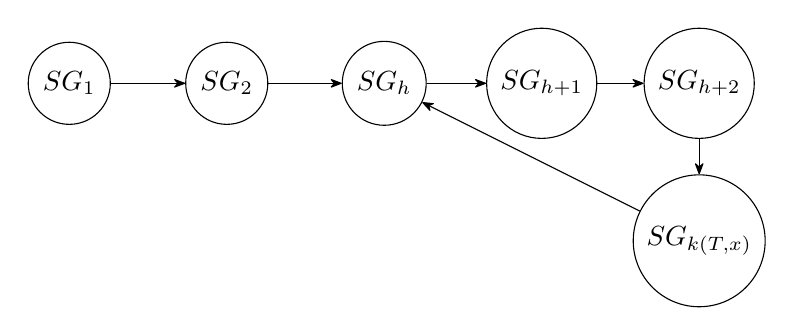
\begin{tikzpicture}[node distance=2cm, every node/.style={draw, circle}, >={Stealth[round]}]
                % Nodes
                \node (A) {$SG_{1}$};
                \node (B) [right of=A] {$SG_{2}$};
                \node (C) [right of=B] {$SG_{h}$};
                \node (D) [right of=C] {$SG_{h + 1}$};
                \node (E) [right of=D] {$SG_{h + 2}$};
                \node (F) [below of=E] {$SG_{k(T, x)}$};
                
                % Edges
                \draw[->] (A) -- (B);
                \draw[->] (B) -- (C);
                \draw[->] (C) -- (D);
                \draw[->] (D) -- (E);
                \draw[->] (E) -- (F);
                \draw[->] (F) -- (C);
            \end{tikzpicture}
        \end{figure}
        Ma $T$ è deterministica, allora, a partire da $SG_{h}$ è possibile eseguire un'unica quintupla (verso $SG_{h + 1}$) ed
        essa viene eseguita tutte le volte in cui $T(x)$ si trova in $SG_{h}$. Quindi, entrambe le volte, avviene una transizione
        verso lo stesso stao globale $SG_{h + 1}$, in questo modo $T(x)$ va in loop e non termina che è contro l'ipotesi che termina.
    }
\end{enumerate}

\newpage
\subsection{Teorema a pag. 4}

Sia $f: \mathbb{N} \rightarrow \mathbb{N}$ una funzione totale e calcolabile.
\begin{itemize}
    \item []{
        Se $L \subseteq \Sigma^{\star}$ è accettato da una macchina di Turing non deterministica $NT$ tale che,
        per ogni $x\in L$, $ntime(NT, x) \leq f(|x|)$ allora $L$ è decidibile.
    }
    \item []{
        Se $L \subseteq \Sigma^{\star}$ è accettato da una macchina di Turing non deterministica $NT$ tale che,
        per ogni $x\in L$, $nspace(NT, x) \leq f(|x|)$ allora $L$ è decidibile.
    }
\end{itemize}

\paragraph*{Dimostrazione:} Poiché $f$ è totale e calcolabile, esiste una macchina di Turing $T_{f}$ trasduttore tale che, per 
ogni $n \in \mathbb{N}$, $T_{f}(n)$ termina con il valore $f(n)$ scritto sul nastro di output. Assumiamo che l'input e l'output 
siano codificati in unario. Sia $L \subseteq \Sigma^{\star}$ un linguaggio accettato da una macchina di Turing $NT$ tale che 
$\forall x \in L,\ ntime(NT, x) \leq f(|x|)$. Deriviamo ora da $NT$ e $T_{f}$ una nuova macchina non deterministica $NT^{'}$ a tre nastri.
\begin{enumerate}
    \item [$N_{1}$:] viene scritto in unario l'input $x \in \Sigma^{\star}$.
    \item [$N_{2}$:] viene scritta la lunghezza di $x$ in unario.
    \item [$N_{3}$:] viene utitlizzato come clock, ovvero viene scritto $f(|x|)$.
\end{enumerate}
La computazione $NT^{'}$ consiste di 3 fasi:
\begin{enumerate}
    \item [FASE 1:]{
        $NT^{'}(x)$ scrive $|x|$ su $N_{2}$ in unario. Una volta letto $\square$ su $N_{1}$, le testine di $N_{1}$ e $N_{2}$
        vengono riposizionate sul carattere più a sinistra.
    }
    \item [FASE 2:]{
        Simula $T_{f}(|x|)$, usando $N_{2}$ come nastro di input e $N_{3}$ come nastro di output. Essa termina scrivendo il valore di 
        $f(|x|)$ su $N_{3}$ e riavvolge la testina.
    }
    \item [FASE 3:]{
        Simula i primi $f(|x|)$ passi della computazione, utilizzando $N_{1}$ come input e nastro di lavoro e $N_{3}$ come clock,
        ovvero come contatore del numero di istruzioni eseguite. Fino a quando viene letto 1 su $N_{3}$ viene eseguita un'istruzione di
        $NT(x)$ e la testina di $N_{3}$ viene spostata a destra. Se $NT(x)$ raggiunge $q_{A}$ o $q_{R}$, $NT^{'}(x)$ termina nel 
        medesimo stato. Se viene letto $\square$ su $N_{3}$, $NT^{'}(x)$ termina in $q_{R}$.
    }
\end{enumerate} 

Poiché $f$ è calcolabile e totale e poiché la simulazione della computazione $NT(x)$ nella terza fase viene forzatamente terminata,
se non ha terminato entro $f(|x|)$ passi, tutte le computazioni di $NT^{'}$ terminano.

\begin{itemize}
    \item {
        Se $x\in L$ allora poiché $NT$ accetta $x$ in $f(|x|)$ passi, nella terza fase termina in $q_{A}$ prima che venga
        letto $\square$.
    }
    \item {
        Se $x\notin L$ allora o $NT(x)$ termina in $q_{R}$ durante la terza fase e di conseguenza anche $NT^{'}(x)$ termina in $q_{R}$,
        oppure viene letto $\square$, ovvero $NT(x)$ non ha accettato $x$ in $f(|x|)$ passi e dunque $NT^{'}(x)$ rigetta.
    }
\end{itemize}
Questo dimostra che $NT^{'}$ decide $L$ e dunque che $L$ è decidibile.
\subsection{Teorema a pag. 10}

Per ogni funzione totale calcolabile $f: \mathbb{N} \rightarrow \mathbb{N}$ 
$$DTIME[f(n)] \subseteq NTIME[f(n)]\ \land\ DSPACE[f(n)] \subseteq NSPACE[f(n)]$$ 

\paragraph*{Dimostrazione:} Una macchina di Turing deterministica è una particolare macchina di Turing non deterministica 
avente grado di non determinismo pari a 1, inoltre ogni parola decisa in $k$ passi e anche accettata in $k$ passi 
(ogni parola decisa in $k$ celle e anche accettata in $k$ celle).

\newpage
\subsection{Teorema a pag. 10}

Per ogni funzione totale calcolabile $f: \mathbb{N} \rightarrow \mathbb{N}$ 

$$DTIME[f(n)] \subseteq DSPACE[f(n)]\ \land\ NTIME[f(n)] \subseteq NSPACE[f(n)]$$ 

\paragraph*{Dimostrazione:} Segue dal teorema:
$$dspace(T, x) \leq dtime(T, x)\dots$$
Sia $L \subseteq \Sigma^{\star}$ tale che $L \in DTIME[f(n)]$. Allora esiste $T$ che decide $L$ e tale che 
$\forall x\in \Sigma^{\star}$, $dtime(T, x) \in O(f(|x|))$. Poiché $dspace(T, x) \leq dtime(T, x) \in O(f(|x|))$,
allora $dspace(T, x) \in O(f(|x|))$, dunque $L \in DSPACE(f(|x|))$.\\ Analogamente per $NTIME[f(n)] \subseteq NSPACE[f(n)]$.

\subsection{Teorema a pag. 11}

Per ogni funzione totale calcolabile $f: \mathbb{N} \rightarrow \mathbb{N}$ 

$$DSPACE[f(n)] \subseteq DTIME[2^{O(f(n))}]\ \land\ NSPACE[f(n)] \subseteq NTIME[2^{O(f(n))}]$$

\paragraph*{Dimostrazione:} Segue dal teorema:
$$\dots dtime(T, x) \leq dspace(T, x)|Q|(|\Sigma| + 1)^{dspace(T, x)}$$
Sia $L \subseteq \Sigma^{\star}$ tale che $L \in DSPACE[f(n)]$. Allora, esiste una machina di Turing $T$ deterministica $T$
che decide $L$ e tale che, per ogni $x \in \Sigma^{\star}$, $dspace(T, x) \in O(f(|x|))$. Poiché:

Supponiamo che $\Sigma = \{0, 1\}$

\[
    \begin{aligned}[t]
    dtime(T, x) &\leq dspace(T, x)|Q|(|\Sigma| + 1)^{dspace(T, x)} \\
                 &\leq dspace(T, x)|Q|3^{dspace(T, x)}\\
                 &\leq 2^{\log(dspace(T,x))}\ |Q|\ 2^{\log(3)dspace(T, x)}\\
                 &\leq |Q|2^{\log(dspace(T,x))\ +\ \log(3)dspace(T, x)}\\
                 &\leq |Q|2^{(1 + \log(3))dspace(T, x)}
    \end{aligned}
\]

Allora $dtime(T, x)\in O(2^{O(f(|x|))})$ e dunque $L\in DTIME[2^{O(f(|x|))}]$

\subsection{Teorema a pag. 11}

Per ogni funzione totale calcolabile $f: \mathbb{N} \rightarrow \mathbb{N}$ 
$$DTIME[f(n)] = coDTIME[f(n)]\ \land\ DSPACE[f(n)] = coDSPACE[f(n)]$$

\paragraph*{Dimostrazione:} $\forall L \in DTIME[f(n)]$, esiste $T$ che decide $L$ e $dtime(T, x) \in O(f(|x|))$. 
Da $T$ deriviamo $T^{c}$ con input $x \in \Sigma^{\star}$ e $Q_{f} = \{q_{A}^{c}, q_{R}^{c}\}$ che decide $L^{c}$ nel seguente modo:

\begin{enumerate}
    \item [FASE 1:] Simula $T(x)$
    \item [FASE 2:]{
        \begin{itemize}
            \item Se $T(x) = q_{A}$, allora $T^{c}(x) = q_{R}$
            \item Se $T(x) = q_{R}$, allora $T^{c}(x) = q_{A}$
        \end{itemize}
    }
\end{enumerate}
Dunque $L^{c} \in DTIME[f(n)]$.\\
Analogamente possiamo dimostrare che un qualsiasi linguaggio $L \in coDTIME[f(n)]$. Di conseguenza che $DTIME[f(n)] = coDTIME[f(n)]$.
Dimostrazione analoga per $DSPACE[f(n)] = coDSPACE[f(n)]$.
\newpage
\subsection{Teorema a pag. 14}

Sia $f: \mathbb{N} \rightarrow \mathbb{N}$ una funzione time-constructible (space-constructible.).
\begin{itemize}
    \item []{
        Allora, per ogni $L \in NTIME[f(n)]$, si ha che $L$ è decidibile in tempo non deterministico in $O(f(n))$.
    }
    \item []{
        Allora, per ogni $L \in NSPACE[f(n)]$, si ha che $L$ è decidibile in spazio non deterministico in $O(f(n))$.
    }
\end{itemize}

\paragraph*{Dimostrazione:} Sia $f: \mathbb{N} \rightarrow \mathbb{N}$ una funzione time-constructible. Allora esiste
una macchina di Turing di tipo trasduttore $T_{f}$ che, avendo scritto sul nastro di input/lavoro $n \in \mathbb{N}$ in 
unario, in $O(f(n))$ passi scrive sul nastro di output il valore di $f(n)$ in unario. Sia $L \in NTIME[f(n)]$. Allora 
esiste una $NT$ che accetta $L$ e tale che, per ogni $x \in L$, $ntime(NT, x) \in O(f(|x|))$. Definiamo ora da $T_{f}$
e $NT$, la macchina $NT^{'}$ con input $x \in L$ che opera nel seguente modo:

\begin{itemize}
    \item [FASE 1:] Scrive su $N_{2}$, $|x|$ in unario. 
    \item [FASE 2:] Simula $T_{f}(x)$ e scrive il risulato in unari su $N_{3}$.
    \item [FASE 3:] {
        Finché legge 1 su $N_{3}$ esegue una istruzione di $NT(x)$ su $N_{1}$. 
        \begin{itemize}
            \item Se termina in $q_{A}$, allora $NT^{'}(x) = q_{A}$.
            \item Altrimenti sposta la testina a destra su $N_{3}$
        \end{itemize}
    }
    \item [FASE 4:] Se legge $\square$ su $N_{3}$ allora rigetta.
\end{itemize}

\begin{itemize}
    \item La fase 1 termina in $O(|x|)$ passi.
    \item la fase 2 termina in $O(f(|x|))$ passi, in quanto $f$ è time-constructible.
    \item La fase 3 termina in $O(f(|x|))$ passi, in quanto $\forall x \in \Sigma^{\star}$, $ntime(NT^{'}, x) \in O(f(|x|))$.
\end{itemize}

Dunque, $NT^{'}(x)$ decide $L,\ \forall x \in \Sigma^{\star}$, e $ntime(NT^{'}, x) \in O(f(|x|))$. 

\subsection{Teorema a pag. 14}

Per ogni funzione $f: \mathbb{N} \rightarrow \mathbb{N}$ time-constructible, $$NTIME[f(n)] \subseteq DTIME[2^{O(f(n)}]$$

\paragraph*{Dimostrazione:} 

Sia $L \in \Sigma^{\star}$ tale che $L \in NTIME[f(n)]$, allora esistono una macchina di Turing $NT$ che accetta $L$ e una 
costante $h$ tali che $\forall x \in L,\ ntime(NT, x) \leq hf(|x|)$. Poiché $f$ è time-constructible, esiste una macchina 
di Turing deterministica $T_{f}$ con inpun la rappresentazione in unario di $n \in \mathbb{N}$, che calcola il valore di 
$f(n)$ in unario in tempo $O(f(n))$. Indichiamo con $k$ il grado di non determinismo di $NT$ e definiamo $T$ deterministica
che simuli $NT$ con input $x \in \Sigma^{\star}$ che opera nel seguente modo:

\begin{itemize}
    \item [FASE 1:] Scrive su $N_{2}$, $|x|$ in unario.
    \item [FASE 2:] {
        Simula $T_{f}(|x|)$ e scrive su $N_{3}$ l'output $hf(|x|)$ in unario.
    }
    \item [FASE 3:] {
        Per ogni computazione deterministica $\alpha(x)$ in $NT(x)$:
        \begin{itemize}
            \item Finché legge 1 su $N_{3}$ esegue un'istruzione lungo $\alpha(x)$.
            \item Se $\alpha(x) = q_{A}$ allora $T(x) = q_{A}$.
            \item Altrimenti sposta la testina a destra su $N_{3}$.
            \item Se legge $\square$ si sposta sul primo 1 a sinistra e passa alla prossima computazione deterministica $\alpha(x)$ se esiste.
        \end{itemize}
    }
    \item [FASE 4:] Rigetta
\end{itemize}

\begin{itemize}
    \item La fase 1 termina in $O(f(|x|))$ passi.
    \item La fase 2 termina in $O(hf(|x|)) = O(f(|x|))$ passi.
    \item La fase 3 termina in $O(f(|x|)k^{hf(x)})$ poiché esegue ogni computazione deterministica di $NT(x)$
\end{itemize}

Dunque, $$dtime(T, x) \in O(f(|x|)k^{hf(x)}) \subseteq{O(2^{O(f(|x|))})}$$

\subsection{Teorema a pag. 20}

Siano $C$ e $C^{'}$ due classi di complessità tali che $C^{'} \subseteq C$. Se $C^{'}$ è chiusa rispetto ad una $\pi$-riduzione
allora, per ogni linguaggio $L$ che sia $C$-completo rispetto a tale $\pi$-riduzione, $L \in C^{'}$ se e solo se $C = C^{'}$.

\paragraph*{Dimostrazione:}

\begin{itemize}
    \item [$\Leftarrow$)] Se $C = C^{'}$ allora $L \in C^{'}$.
    \item [($\Rightarrow$]{
        Sia $L \in C^{'}$. Poiché $L$ è $C$-completo rispetto alla $\pi$-riducibilità, allora per ogni $L_{0} \in C$, 
        $L_{0} \leq_{\pi} L$. Poiché $C^{'}$ è chiusa rispetto alla $\pi$-riduzione, ovvero per ogni altro linguaggio 
        $L^{'}$, $L^{'} \leq_{\pi} L$, allora $L^{'} \in C^{'}$, dunque per ogni linguaggio $L_{0} \in C$, $L_{0} \leq_{\pi} L$,
        allora $L_{0} \in C^{'}$. Quindi $C = C^{'}$.
    }
\end{itemize}

\subsection{Teorema a pag. 21}

La classe \textbf{P} è chiusa rispetto alla riducibilità polinomiale.

\paragraph*{Dimostrazione:}

Sia $L \in \textbf{P}$, allora esistono una macchina di Turing $T$ deterministica e $k \in \mathbb{N}$ tale che $T$ decide $L$ e 
per ogni $x \in \Sigma^{\star}$, $dtime(T, x) \in O(|x|^k)$.

Sia $L^{'}:\ L^{'} \leq_{p} L$, allora esiste una funzione $f: \Sigma^{\star}_{1} \rightarrow \Sigma^{\star}_{2}$ in $\textbf{FP}$
che riduce $L^{'}$ a $L$, con $T_{f}$ trasduttore tale che per ogni $x \in \Sigma^{\star}_{1}$, $T_{f}(x) \in L \Leftrightarrow x \in L^{'}
\land dtime(T_{f}, x) \in O(|x|^c)$.

Da $T$ e $T_{f}$ definiamo $T^{'}$ con input $x$ che opera nel seguente modo:

\begin{itemize}
    \item [FASE 1:] Simula $T_{f}(x)$ e scrive l'output $y$ su $N_{2}$.
    \item [FASE 2:] {
        Simula $T(y)$:
        \begin{itemize}
            \item Se termina in $q_{A}$ allora $T^{'}$ accetta.
            \item Se termina in $q_{R}$ allora $T^{'}$ rigetta.
        \end{itemize}
    }
\end{itemize}

Dato che $f$ è una riduzione da $L^{'}$ a $L$, quindi $f(x) \in L \Leftrightarrow x \in L^{'}$, quindi $T^{'}$ termina per 
ogni input $x \in \Sigma^{\star}$ e accetta $\Leftrightarrow$ $T(f(x))$ accetta, ossia $\Leftrightarrow\ f(x) \in L$.

Resta da mostrare che $T^{'}(x)$ opera in tempo polinomiale in $|x|$. La simulazione di $T_{f}(x)$ richiede 
$dtime(T_{f}, x) \leq |x|^c$ e la simulazione di $T(f(x))$ richiede $dtime(T, f(x)) \leq |f(x)|^k$.

\[
    \begin{aligned}[t]
        dtime(T^{'}, x) &\leq |x|^c + f(|x|)^k\footnote{$f(|x|)^k = |y|^k$ che per il teorema: $dspace(T, x) \leq dtime(T, x)$, 
        $|y|^k \leq (|x|^c)^k = |x|^{ck}$} \\
                &\leq |x|^c + |x|^{ck}\\
                &\Rightarrow dtime(T^{'}, x) \in O(|x|^{ck})
    \end{aligned}
\]

Poiché $c$ e $k$ sono costanti, allora risulta che \textbf{P} è chiusa rispetto la riducibilità polinomiale dato che $L^{'} \in \textbf{P}$.

\subsection{Teorema a pag. 21}

Le classi \textbf{NP, PSPACE, EXPTIME, NEXPTIME}, sono chiuse rispetto alla riducibilità polinomiale.

\paragraph*{Dimostrazione:} 

\begin{itemize}
    \item [\textbf{NP}]
    \item [\textbf{PSPACE}]
    \item [\textbf{EXPTIME}]
    \item [\textbf{NEXPTIME}]
\end{itemize}

\subsection{Corollario a pag. 21}

Se \textbf{P $\neq$ NP} allora, per ogni linguaggio \textbf{NP}-completo $L$, $L \notin \textbf{P}$.

\paragraph*{Dimostrazione:} 

Supponiamo che $L$ sia un linguaggio \textbf{NP}-completo e che $L \in \textbf{P}$. Poiché $L$ è \textbf{NP}-completo, per ogni
linguaggio $L^{'} \in \textbf{NP},\ L^{'} \leq L$, ma se $L \in \textbf{P}$, poiché \textbf{P} è chiusa rispetto alla 
riduzione $\leq$, questo implica che, per ogni $L^{'} \in \textbf{NP},\ L^{'} \in \textbf{P}$. Ossia \textbf{P = NP}, 
contraddicendo l'ipotesi.

\subsection{Teorema a pag. 23}

Se \textbf{NP $\neq$ coNP}, allora \textbf{P $\neq$ NP}.

\paragraph*{Dimostrazione ($A\rightarrow B \Leftrightarrow \lnot B \rightarrow \lnot A$): }

Se \textbf{P = NP}, allora \textbf{NP = coP} poiché \textbf{P = coP}. Ma se \textbf{P = NP} $\land$ \textbf{P = coP}, allora 
\textbf{coP = coNP}. Dunque: $$\textbf{\underline{NP} = P = coP = \underline{coNP}}$$ 

\subsection{Teorema a pag. 23}

La classe \textbf{coNP} è chiusa rispetto alla riducibilità polinomiale.

\paragraph*{Dimostrazione: }

Poiché \textbf{NP} è chiusa rispetto alla riducibilità polinomiale
\begin{itemize}
    \item [] Per ogni $L_{2} \in \textbf{NP}$ e per ogni $L_{1}$, se $L_{1} \leq L_{2}$, allora $L_{1} \in \textbf{NP}$.
    \item [$\Rightarrow$] Per ogni $L_{2}^{c} \in \textbf{coNP}$ e per ogni $L_{1}^{c}$, se $L_{1}^{c} \leq L_{2}^{c}$, allora $L_{1}^{c} \in \textbf{coNP}$
\end{itemize}

\subsection{Teorema a pag. 23}

Un linguaggio L è \textbf{NP}-completo se e soltanto se $L^{c}$ è \textbf{coNP}-completo. 

\paragraph*{Dimostrazione: }

\begin{itemize}
    \item [($\Rightarrow$]{
        Sia $L$ un linguaggio \textbf{NP}-completo, allora per definizione di completezza
        \begin{enumerate}
            \item $L \in \textbf{NP}$ allora $L^{c} \in \textbf{coNP}$.
            \item $\forall L_{0} \in \textbf{NP},\ L_{0} \leq L$.
        \end{enumerate}
        Sia $L_{1}$ un qualsiasi linguaggio in \textbf{coNP}, allora $L^{c}_{1} \in \textbf{NP}$. 
        Poiché $L$ è \textbf{NP}-completo, $L_{1}^{c} \leq L$.
        \[
            \begin{aligned}[t]
                &\Rightarrow Esiste\ f \in \textbf{FP}: \forall x \in \Sigma^{\star} [x \in L^{c}_{1} \Leftrightarrow f(x) \in L]\\
                &\Rightarrow Esiste\ f \in \textbf{FP}: \forall x \in \Sigma^{\star} [x \notin L^{c}_{1} \Leftrightarrow f(x) \notin L]\\
                &\Rightarrow Esiste\ f \in \textbf{FP}: \forall x \in \Sigma^{\star} [x \in L_{1} \Leftrightarrow f(x) \in L^{c}]\\
            \end{aligned}
        \]
        In conclusione, $\forall L_{1} \in \textbf{coNP}:\ L_{1} \leq L^{c}$, e quindi $L^{c}$ è \textbf{coNPC}.
    }
    \item [$\Leftarrow$)]{
        Sia $L^{c}$ un linguaggio \textbf{coNP}-completo, allora per definizione di completezza
        \begin{enumerate}
            \item $L^{c} \in \textbf{coNP}$ allora $L \in \textbf{NP}$.
            \item $\forall L_{0}^{c} \in \textbf{coNP},\ L_{0}^{c} \leq L^{c}$.
        \end{enumerate}
        Sia $L_{1}$ un qualsiasi linguaggio in \textbf{NP}, allora $L^{c}_{1} \in \textbf{coNP}$.
        Poiché $L^{c}$ è \textbf{coNP}-completo, $L_{1}^{c} \leq L^{c}$.
        \[
            \begin{aligned}[t]
                &\Rightarrow Esiste\ f \in \textbf{FP}: \forall x \in \Sigma^{\star} [x \in L^{c}_{1} \Leftrightarrow f(x) \in L^{c}]\\
                &\Rightarrow Esiste\ f \in \textbf{FP}: \forall x \in \Sigma^{\star} [x \notin L^{c}_{1} \Leftrightarrow f(x) \notin L^{c}]\\
                &\Rightarrow Esiste\ f \in \textbf{FP}: \forall x \in \Sigma^{\star} [x \in L_{1} \Leftrightarrow f(x) \in L]\\
            \end{aligned}
        \]
        In conclusione, $\forall L_{1} \in \textbf{NP}:\ L_{1} \leq L$, e quindi $L$ è \textbf{NPC}.
    }
\end{itemize}

\newpage
\subsection{Teorema a pag. 24}

Se esiste un linguaggio $L$ \textbf{NP}-completo tale che $L \in \textbf{coNP}$, allora \textbf{NP = coNP}.

\paragraph*{Dimostrazione: }

$L$ è \textbf{NP}-completo, allora per definizione di completezza
\begin{enumerate}
    \item $L \in \textbf{NP}$.
    \item $\forall L_{1} \in \textbf{NP},\ L_{1} \leq L$.
\end{enumerate}

\begin{itemize}
    \item [$\subseteq$]{
        Se $L \in \textbf{coNP}$ allora $\forall L_{1} \in \textbf{NP},\ L_{1} \leq L$, ma \textbf{coNP} è chiusa ripsetto 
        alla riducibilità polinomiale ovvero [$L_{2} \in \textbf{coNP},\ L_{1} \leq L_{2},\ \Rightarrow\ L_{1} \in \textbf{coNP}$],
        allora, per ogni $L_{1} \in \textbf{NP}$ si ha che $L_{1} \leq L$, e $L \in \textbf{coNP}$. Dunque, per la chisura di \textbf{coNP},
        $L_{1} \in \textbf{coNP}$, quindi \textbf{NP $\subseteq$ coNP}. 
    }
    \item [$\supseteq$]{
        Poiché $L \in \textbf{coNP}$, allora $L^{c} \in \textbf{NP}$, ma poiché $L$ è \textbf{NP}-completo, allora $L^{c}$ è
        \textbf{coNP}-completo, quindi $\forall L^{'} \in \textbf{coNP},\ L^{'} \leq L^{c}$. Ma \textbf{NP} è chiusa rispetto alla 
        riducibilità polinomiale, ovvero [$L_{2} \in \textbf{NP},\ L_{1} \leq L_{2},\ \Rightarrow\ L_{1} \in \textbf{NP}$],
        allora, per ogni $L^{'} \in \textbf{coNP},\ L^{'} \leq L^{c}$ e $L^{c} \in \textbf{NP}$. Dunque, per la chiusura di \textbf{NP}, 
        $L^{'} \in \textbf{NP}$, quindi \textbf{coNP $\subseteq$ NP}.   
    }
\end{itemize}

In conclusione, se $L$ è \textbf{NP}-completo $\land$ $L \in \textbf{coNP}$, allora \textbf{NP = coNP}.
\section{Teoremi Dispensa 7}

\subsection{Teorema a pag. 9}

Sia $\Gamma = \langle I_{\Gamma},\ S_{\Gamma},\ \pi_{\Gamma} \rangle$ un problema decisionale e sia $\chi: I_{\Gamma} \rightarrow \Sigma^*$
una sua codifica ragionevole, se $\chi(I_{\Gamma}) \in \textbf{P}$\footnote{Questo perché la decisione del linguaggio delle istanze
deve richiedere "poche risorse", altrimenti non sappiamo dire nulla riguardo il linguaggio del problema complemento.}, allora 
\[
L_{\Gamma}(\chi) \in \textbf{NP} \Rightarrow L_{\Gamma^c}(\chi) \in \textbf{coNP} 
\]

\paragraph*{Dimostrazione:}

\begin{itemize}
    \item []{
        Poiché $\chi(I_{\Gamma}) \in \textbf{P}$, allora $\exists,\ T,\ h \in \mathbb{N}$ tale che $\forall x \in \Sigma^*$
        $T(x) =
        \begin{cases} 
            & q_{A} \Leftrightarrow x\in \chi(I_{\Gamma})\\
            & q_{R} \Leftrightarrow x\notin \chi(I_{\Gamma})\\
        \end{cases}$ 
        $\land\ dtime(T, x) \leq |x|^h$.
    }
    \item []{
        Se $L_{\Gamma}(\chi) \in \textbf{NP}$ allora $\exists\ NT, k \in \mathbb{N}$ tale che 
        \[
            \forall x \in L_{\Gamma}(\chi)\ NT(x) = q_{A}\ \land\ \forall x \notin L_{\Gamma}(\chi)\ NT(x)
            \neq q_{A}\ \land\ ntime(NT, x) \leq |x|^k
        \] 
    }
    \end{itemize}
    
Da $T$ e $NT$ deriviamo $NT^{'}$ con input $x \in \Sigma^*$ che opera nel seguente modo:
\begin{itemize}
    \item [FASE 1: ] Simula $T(x)$. Se $T(x) = q_{R}$ allora $NT^{'} = q_{A}$. Se $T(x) = q_{A}$ allora esegui la fase 2.
    \item [FASE 2: ] Simula $NT(x)$.
\end{itemize}

Quindi $NT^{'}$ accetta se e soltanto se $x \in L_{\Gamma} \lor x \notin \chi(I_{\Gamma})$, ossia se e soltanto se $x \in (L_{\Gamma^c})^c$.
Dunque $NT^{'}$ accetta $L_{\Gamma^c}^c$, e $ntime(NT^{'}, x) \leq |x|^{\max(h, k)}$, quindi $(L_{\Gamma^c})^c \in \textbf{NP} \Rightarrow L_{\Gamma^c} \in \textbf{coNP}$.

\begin{figure}[h]
    \centering
    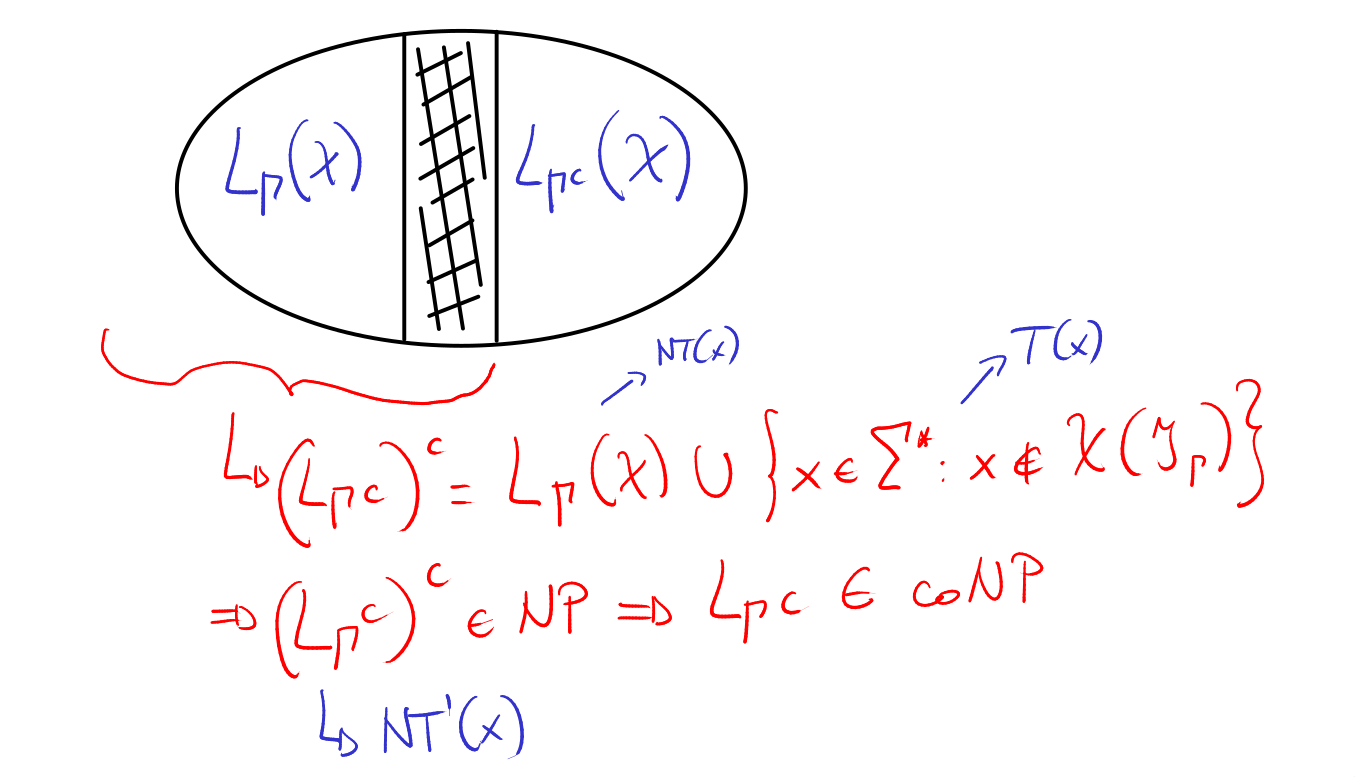
\includegraphics[width=0.8\textwidth]{../img/th7.png}
    \caption{Schema grafico della dimostrazione}
  \end{figure}
\section{Teoremi Dispensa 9}

\subsection{Teorema a pag. 8}

Un linguaggio $L \subseteq \Sigma^{\star}$ è in \textbf{NP} \underline{se è soltanto se}\footnote{Questo è da dimostrare}
esistono una macchina di Turing deterministica $T$ che opera in tempo polinomiale e due costanti $k, h \in \mathbb{N}$ tali che, 
per ogni $x \in \Sigma^{\star},\ x \in L \Leftrightarrow \exists y_{x} \in \{0, 1\}^{\star}:\ |y_{x}| \leq |x|^k
\land T(x, y_{x}) = q_{A} \land dtime(T, x, y_{x}) \leq |x|^h$

\paragraph*{Dimostrazione: }

\begin{itemize}
    \item [($\Rightarrow$]{
        Sia $L \subseteq \Sigma^{\star}$ un linguaggio in \textbf{NP}, allora esistono una macchina di Turing non 
        deterministica $NT$ e un intero $h \in \mathbb{N}$ tale che $NT$ accetta $L$ e, per ogni, $x \in L,\ ntime(NT, x) \leq |x|^h$.
        
        Questo significa che $\forall x \in L$ esiste una sequenza di quintuple che eseguite a partire dallo stato globale inziale $SG_{0}$ 
        porta ad uno stato globale di accettazione. 

        Allora, $p_{i} = \langle q_{i1},\ s_{i1},\ s_{i2},\ q_{i2},\ m_{i} \rangle$ è la $i-esima$ quintupla 
        della sequenza $y(x)$, definita come segue:
        $$y(x) =\ q_{11},\ s_{11},\ s_{12},\ q_{12},\ m_{1}\ -\ q_{21},\ s_{21},\ s_{22},\ q_{22},\ m_{2}\ -\ \dots\ -\ q_{(n^{k})1},\ s_{(n^{k})1},\ s_{(n^{k})2},\ q_{(n^{k})2},\ m_{(n^{k})}$$
        è la sequenza di quintuple che rappresentano una computazione deterministica accettante.\footnote{Adesso il Genio non ci da più una quintupla per volta, ma una sequenza di quintuple che però, devono essere verificate.}

        Definiamo ora una macchina deterministica $\overline{T}$ che ha il ruolo di verificare la sequenza di quintuple $y_{x}$ scelta dal genio. Dunque $\overline{T}$ è 
        detto \textbf{verificatore} ed opera nel seguente modo:
        \begin{enumerate}
            \item $\overline{T}$ verifica che $y$ sia nella forma descritta sopra, se non è così, rigetta.
            \item $\overline{T}$ verifica che, per ogni $1 \leq i \leq n^k,\ \langle q_{i1},\ s_{i1},\ s_{i2},\ q_{i2},\ m_{i} \rangle \in P$, se non è così, allora rigetta.
            \item $\overline{T}$ verifica che $q_{11} = q_{0}$ e $q_{(n^k)2} = q_{A}$, se così non è, rigetta.
            \item $\overline{T}$ verifica che, per ogni $2 \leq i \leq n^k,\ q_{i1} = q_{(i - 1)2}$, se così non è, rigetta.
            \item $\overline{T}$ simula la computazione di $NT(x)$ descritta da $y$. Verifica se ogni quintupla può essere eseguita, se sì la esegue, altrimenti rigetta.
            \item $\overline{T}$ accetta.
        \end{enumerate}

        Dunque, se $x \in L$, allora $y(x)$ è la codifica di $NT(x)$ accettante che è costituita da al più $|x|^k$ passi. 
        Dunque, se $x \in L$, allora $|y(x) \in O(|x|^k)|$ e quindi $\overline{T}$ opera in tempo polinomiale in $|x|$.

        Se $x \in L,\ y_{x}$ prende il nome di \textbf{certificato} per $x$. Dunque $x \in L \Leftrightarrow\ \exists y(x) \in [\Sigma \cup Q \cup \{-, s, f, d\}^{\star}]$ tale che $\overline{T}(x, y_{x})$ accetta.
    }
    \item [$\Leftarrow$)]{
        Sia $L \subseteq \Sigma^{\star}$ un linguaggio per il quale esistono una macchina di Turing deterministica $T$ che opera in 
        tempo polinomiale e una costante $k \in \mathbb{N}$ tali che, $\forall x \in \Sigma^{\star},\ x \in L \Leftrightarrow \exists y_{x} \in \{0, 1\}^{\star}$, tale che $|y_{x}| \leq |x|^k \land T(x, y_{x})$ accetta.

        Dobbiamo dimostrare che $\exists NT$ e $a \in \mathbb{N}$ tale che, $\forall x \in L,\ NT(x)$ accetta e $ntime(NT, x) \in O(|x|^a)$. $NT$ opera come segue:
        \begin{itemize}
            \item [FASE 1: ] $NT$ sceglie non determisticamente una parola binaria $y$ di lunghezza $|y| \leq |x|^k$.
            \item [FASE 2: ] $NT$ invoca $T(x, y)$ e, se $T(x, y)$ accetta entro $O(|x|^h)$ passi allora accetta.
        \end{itemize}

        \textbf{NOTA:} $|x|^k$ è time-constructible, ovvero essite una macchina $T_{f}$ trasduttore che calcola $|x|^k$ e $dtime(T_{f}, x) \leq |x|^k$.
    
        \begin{algorithm}[ht]
            \begin{algorithmic}[1]
                \Procedure{NT-FASE-1}{
                    $x \in \Sigma^{\star}$
                }
                    \State $B \gets T_{f}(|x|)$
                    \State $i \gets 1$
                    \While{$i \leq B$} \textbf{begin}
                        \State \underline{scegli} $y[i]$ nell'insieme $\{0, 1\}$
                        \State $i \gets i + 1$
                    \EndWhile \textbf{end}
                    \State $y \gets y[1] \oplus y[2] \oplus \dots \oplus y[B]$
                    \State \Return $y$
                \EndProcedure

                \Procedure{NT-FASE-2}{
                    $x \in \Sigma^{\star}$
                }
                    \State $y_{x} \gets NT-FASE-1(x)$ \Comment{$O(|x|^k)$}
                    \State $q \gets T(x, y_{x})$ \Comment{$O(|x|^h)$}
                    \State \Return $q$
                \EndProcedure
            \end{algorithmic}
        \end{algorithm}
        
        \begin{itemize}
            \item {
                Se $x \in L$ allora $\exists y_{x} \in \{0, 1\}^{\star}:\ |y_{x}| \leq |x|^k \land T(x, y_{x}) = q_{A}$, allora 
                esiste  una sequenza di scelte che genera $y_{x}$, allora nella $FASE\ 2$, $T(x, y_{x})$ accetta entro $|x|^h$ passi, 
                allora $NT(x)$ corrisponde alla sequenza di scelte che ha generato $y_{x}$ e accetta. Questo dimostra che se $x \in L$, allora 
                $NT(x)$ accetta.
            }
            \item {
                Se $x \notin L$ allora non esiste alcuna $y_{x} \in \{0, 1\}$, non esiste alcuna $y(x)$ tale che $|y(x)| \leq |x|^k \land T(x, y_{x}) = q_{A}$.
                Dunque, qualunque sia la sequenza di scelte per generare  $y$, $T(x, y)$ non accetta. Quindi se $x \notin L$, allora $NT(x)$ non accetta. 
            }
        \end{itemize}
    }
\end{itemize}

Questo dimostra che $L \in \textbf{NP}$

\newpage
\subsection{Teorema a pag. 14}

Sia $\Gamma_{1} \in \textbf{NP} \land \exists\ \Gamma_{2} \in \textbf{NPC} \land \Gamma_{2} \leq \Gamma_{1}$, allora 
$\Gamma_{1}$ è \textbf{NPC}.

\paragraph*{Dimostrazione: }

\begin{itemize}
    \item []{
        Sia $\Gamma_{2}$ un problema \textbf{NPC} tale che $\Gamma_{2} \leq \Gamma_{1}$, allora $\exists\ f_{21}:\ I_{\Gamma_{2}} \rightarrow I_{\Gamma_{1}}$
        tale che $f_{21} \in \textbf{FP}$ e per ogni $x \in I_{\Gamma_{2}},\ [x \in \Gamma_{1} \Leftrightarrow f_{21}(x) \in \Gamma_{1}]$, 
        ovvero $$\exists\ T_{21}, k:\ \forall x \in I_{\Gamma_{2}},\ [x \in \Gamma_{1} \Leftrightarrow T_{21}(x) \in \Gamma_{1} \land\ dtime(T_{21}, x) \leq |x|^k]$$
    }
    \item []{
        Poiché $\Gamma_{2}$ è \textbf{NPC}, per ogni problema $\Gamma_{3} \in \textbf{NP}$ si ha che $\Gamma_{3} \leq \Gamma_{2}$, e dunque esiste una funzione $f_{32}:\ \Gamma_{3} \Rightarrow \Gamma_{2}$
        tale che $f_{32} \in \textbf{FP}$ e per ogni $z \in I_{\Gamma_{3}},\ [z \in \Gamma_{3} \Leftrightarrow f_{32}(z) \in \Gamma_{2}]$, ovvero 
        $$\exists\ T_{32}, h: \forall z \in I_{\Gamma_{3}},\ [z \in \Gamma_{2} \Leftrightarrow T_{32}(z) \in \Gamma_{2} \land\ dtime(T_{32}, z) \leq |x|^h]$$
    }
\end{itemize}
Da $T_{21}$ e $T_{32}$ definiamo $T_{31}$ con input $z \in I_{\Gamma_{3}}$ che opera nel seguente modo:

\begin{itemize}
    \item [FASE 1: ] Simula $T_{32}(z) = x$
    \item [FASE 2: ] Simula $T_{21}(x) = y$
    \item [FASE 3: ] Scrivi sul nastro di output $y$
\end{itemize}

Sia $z \in I_{\Gamma_{3}}$, allora $z \in \Gamma_{3} \Leftrightarrow f_{32}(z) \in \Gamma_{2}$ e inoltre, $f_{32}(z) \in \Gamma_{2} \Leftrightarrow f_{21}(f_{32}(z)) \in \Gamma{1}$.
Se indichiamo con $f_{31}$ la composizione delle funzionie $f_{32}$ e $f_{21}$, questo dimostra che $f_{31}$ è una riduzione da $\Gamma_{3}$ a $\Gamma_{1}$.

Resta da dimostrare che la macchina $T_{32}$ opera in tempo polinomiale. 
\[
\forall z \in I_{\Gamma_{3}}:\ [dtime(T_{31}, z) = dtime(T_{32}, z) + dtime(T_{21}, x) \leq |z|^h + |x|^k \leq |z|^{hk}]    
\]

Questo dimostra che $\Gamma_{1}$ è \textbf{NPC}.


\end{flushleft}
\end{document}

